\section{A certified double radial turning-point bifurcation}
\label{turn:sec:main}

The local radial problem has a second layer of degeneracy.  The
manuscript proves that the first nonconstant coefficient of the
normalized radius changes sign at a unique outer-order threshold for
each inner order $0<b<1$.  It subsequently proves opposite signs of the
next coefficient at two points of that threshold curve, and locates a
possible transition numerically \cite{Repo}.  Its final question in
\texttt{05-real-turning.tex} asks for the higher-order behavior at such a
transition.  We certify one transition, determine its next coefficient,
and prove that nearby normalized-radius curves can have two small-radius
turning points: a minimum followed by a maximum.

The conclusion is local in both the parameters and the radius.  It
does not settle the number of quartic transitions over the entire
interval $0<b<1$, nor exclude additional turning points farther from
the origin.  These distinctions matter because an initial Taylor
coefficient, even with a proved sign, does not control the whole disk.

\subsection{An exact finite recurrence to every radial order}
\label{turn:sec:recurrence}

For $a,b>0$, put
\begin{equation}
 F_{a,b}(z)=\sum_{n=2}^{\infty}p_n(a,b)z^n,
 \qquad
 p_n(a,b)=\frac{H_{n-1}^{(b)}}{n^a},
 \qquad
 H_{n-1}^{(b)}=\sum_{j=1}^{n-1}j^{-b}.
 \label{turn:eq:def}
\end{equation}
Let $\theta_{a,b}(\rho)$ denote the local solution near $\pi/2$ of
\[
 \operatorname{Im}F_{a,b}(\rho e^{i\theta})=0,
\]
for positive sufficiently small $\rho$, and set
\begin{equation}
 \eta_{a,b}(\rho)=\frac{\cos\theta_{a,b}(\rho)}{\rho},
 \qquad t=\rho^2.
 \label{turn:eq:eta}
\end{equation}
The radius $\rho$ in this section is a disk radius.  We write the
analytic extension in the squared radius as
$\eta_{a,b}(\rho)=\Phi(a,b,t)$.

\begin{proposition}[An all-orders finite coefficient identity]
\label{turn:prop:recurrence}
For $m\ge0$, define the polynomial
\begin{equation}
 E_m(y)=\sum_{n=m+2}^{2m+3}
  (-1)^{n-m-2}\binom{m+1}{n-m-2}
  2^{2m+3-n}p_n y^{2m+3-n}.
 \label{turn:eq:Em}
\end{equation}
Locally in $(a,b,t)$, the normalized-radius equation is the convergent
analytic identity
\begin{equation}
 \sum_{m=0}^{\infty}t^mE_m\bigl(\Phi(a,b,t)\bigr)=0.
 \label{turn:eq:implicit}
\end{equation}
There is a unique local analytic solution with
$\Phi(a,b,0)=\mu:=p_3/(2p_2)$.  If
\[
 \Phi(a,b,t)=\mu+\sum_{j\ge1}c_j(a,b)t^j,
\]
then the exact recursive identity is
\begin{equation}
 c_j=-\frac{1}{2p_2}[t^j]
 \sum_{m=1}^{j}t^m E_m\left(
   \mu+\sum_{\ell=1}^{j-1}c_\ell t^\ell\right).
 \label{turn:eq:coefficient-recursion}
\end{equation}
In particular, $c_j$ depends only on $p_2,\ldots,p_{2j+3}$.
\end{proposition}

\begin{proof}
For $\theta$ near $\pi/2$, divide the imaginary-part equation by
$\rho^3\sin\theta$ and use
$\sin(n\theta)=\sin\theta\,U_{n-1}(\cos\theta)$.  The finite Chebyshev
identity is
\[
 U_{n-1}(x)=\sum_{h=0}^{\lfloor(n-1)/2\rfloor}
  (-1)^h\binom{n-1-h}{h}(2x)^{n-1-2h}.
\]
After substituting $x=\rho y$, a summand in
$p_n\rho^{n-3}U_{n-1}(\rho y)$ has radius exponent
$2n-4-2h$.  It contributes to $t^m$ exactly when $h=n-2-m$.
The inequalities $0\le h\le\lfloor(n-1)/2\rfloor$ are equivalent to
$m+2\le n\le2m+3$.  Substitution gives precisely
\eqref{turn:eq:Em}.

This is an analytic identity, not merely a formal rearrangement.
On a compact complex neighborhood of fixed positive $(a,b)$, the
coefficients $p_n(a,b)$ are analytic and grow at most polynomially in
$n$.  The Chebyshev recurrence bounds $U_{n-1}(\rho y)$ exponentially
in $n$, uniformly when $y$ stays bounded and $\rho$ is sufficiently
small.  Hence the normalized series converges locally uniformly.  The
apparent negative power in its $n=2$ term cancels, leaving $2p_2y$;
all remaining powers of $\rho$ are nonnegative and even.  The sum is
therefore jointly analytic in $(a,b,t,y)$.

Now $E_0(y)=2p_2y-p_3$, and $2p_2\ne0$ at real positive parameters.
The analytic implicit-function theorem gives the unique solution
$y=\Phi(a,b,t)$ through $\mu=p_3/(2p_2)$.  For small positive $\rho$,
the angle $\arccos(\rho\Phi(a,b,\rho^2))$ is near $\pi/2$ and solves
the original equation, proving the claimed local interpretation.
Finally, the contribution of $E_0$ to the coefficient of $t^j$ is
$2p_2c_j$.  Since every other term has a factor $t^m$ with $m\ge1$,
its coefficient of degree $j$ uses only the already determined
$c_1,\ldots,c_{j-1}$.  Solving for $c_j$ proves
\eqref{turn:eq:coefficient-recursion}.
\end{proof}

The recurrence makes the finite nature of a local degeneracy test
explicit.  For example, no coefficient of $F_{a,b}$ beyond $p_9$ is
needed to determine the first three nonconstant coefficients of
$\eta$.  This is useful when a small coefficient results from nearly
cancelling terms: one can certify a finite expression directly instead
of estimating derivatives from values of the full boundary function.

\subsection{The sextic coefficient}
\label{turn:sec:sextic}

Write
\begin{equation}
 \Phi(a,b,t)=\mu+Kt+Qt^2+Rt^3+O(t^4).
 \label{turn:eq:expansion}
\end{equation}
Thus $K,Q,R$ are respectively the coefficients of
$\rho^2,\rho^4,\rho^6$ in the normalized radius.  Define
\begin{align}
 A(y)&=4p_3y^2-4p_4y+p_5,\notag\\
 B(y)&=8p_4y^3-12p_5y^2+6p_6y-p_7,\notag\\
 C(y)&=16p_5y^4-32p_6y^3+24p_7y^2-8p_8y+p_9.
 \label{turn:eq:ABC}
\end{align}
These are $E_1,E_2,E_3$ in Proposition~\ref{turn:prop:recurrence}.

\begin{proposition}[The first three nonconstant coefficients]
\label{turn:prop:sextic}
The exact coefficient formulas are
\begin{align}
 K&=-\frac{A(\mu)}{2p_2},\notag\\
 Q&=-\frac{A'(\mu)K+B(\mu)}{2p_2},\notag\\
 R&=-\frac{A'(\mu)Q+4p_3K^2+B'(\mu)K+C(\mu)}{2p_2}.
 \label{turn:eq:KQR}
\end{align}
At any simultaneous zero of $K$ and $Q$,
\begin{equation}
 R=-\frac{C(\mu)}{2p_2}.
 \label{turn:eq:Rzero}
\end{equation}
All these quantities are real analytic in positive $(a,b)$.
\end{proposition}

\begin{proof}
Retaining degrees at most three in \eqref{turn:eq:implicit} gives
\[
 0=2p_2\Phi-p_3+tA(\Phi)+t^2B(\Phi)+t^3C(\Phi)+O(t^4).
\]
The coefficients of $t,t^2,t^3$ are respectively
\begin{align*}
 &2p_2K+A(\mu),\\
 &2p_2Q+A'(\mu)K+B(\mu),\\
 &2p_2R+A'(\mu)Q+\tfrac12A''(\mu)K^2+B'(\mu)K+C(\mu).
\end{align*}
Since $A''=8p_3$, their vanishing gives
\eqref{turn:eq:KQR}.  The denominators do not vanish at positive
parameters, so analyticity follows from the finite formulas.
\end{proof}

The manuscript already identifies $K$ and $Q$ and proves that, on
the curve $K=0$, the quartic coefficient has opposite signs at
$b=1/2$ and $b=999/1000$.  The sextic formula supplies the missing
test when both of those earlier coefficients vanish.

\subsection{A unique certified transition in a rational rectangle}
\label{turn:sec:certificate}

Let $\mathcal B$ be the open rectangle with rational endpoints
\begin{align}
 a_-&=1.0014301809614951381293517293,\notag\\
 a_+&=1.0014301809614951381293517295,\notag\\
 b_-&=0.9974937898734204210746055930669,\notag\\
 b_+&=0.9974937898734204210746055930670.
 \label{turn:eq:box}
\end{align}
The many digits here specify an exact, reproducible rational box.
They do not play the role of unproved floating-point approximations.

\begin{theorem}[A nondegenerate quartic transition]
\label{turn:thm:transition}
There is exactly one pair $(a_\dagger,b_\dagger)\in\mathcal B$ such
that $K(a_\dagger,b_\dagger)=Q(a_\dagger,b_\dagger)=0$.
Let $R_0=R(a_\dagger,b_\dagger)$.  Then
\begin{align}
 -3.368744535599044\cdot10^{-11}
  &<R_0<-3.368744535599042\cdot10^{-11},\notag\\
 -8.315139843259675\cdot10^{-10}
  &<\det D(K,Q)<-8.315139843259673\cdot10^{-10}.
 \label{turn:eq:certified-main}
\end{align}
The determinant in the second line is evaluated at the certified pair.
In particular, $(a,b)\mapsto(K,Q)$ is a local real analytic
diffeomorphism there.

The curve $K=0$ is locally a graph $a=a_*(b)$ throughout the
$b$ interval in \eqref{turn:eq:box}.  If
$q_*(b)=Q(a_*(b),b)$, then its zero is unique in that interval, and
\begin{equation}
 4.8702847165970496\cdot10^{-8}
 <q_*'(b_\dagger)<4.8702847165970497\cdot10^{-8}.
 \label{turn:eq:qprime}
\end{equation}
\end{theorem}

\begin{proof}
The accompanying program \texttt{code/certify\_double\_turning.py}
uses only integers and rational numbers.  Its exact interval output is
\texttt{data/double\_turning\_certificate.json}.  We first describe
the elementary arithmetic that makes the certificate a finite proof,
and then explain how its inequalities imply the theorem.

Every interval operation is rounded outward to multiples of
$2^{-256}$.  For integers $1\le n\le9$, write $z=(n-1)/(n+1)$ and use
\[
 \log n=2\sum_{j\ge0}\frac{z^{2j+1}}{2j+1}.
\]
After the first $L=440$ terms, the omitted positive tail is at most
\begin{equation}
 \frac{2z^{2L+1}}{(2L+1)(1-z^2)}.
 \label{turn:eq:log-tail}
\end{equation}
For a rational $0\le x<3$, the Taylor polynomial for $e^x$ through
degree $M=90$ has omitted positive tail at most
\begin{equation}
 \frac{x^{M+1}}{(M+1)!}\frac{1}{1-x/(M+2)}.
 \label{turn:eq:exp-tail}
\end{equation}
These bounds follow respectively by bounding the remaining denominators
from below and the ratio of consecutive omitted terms from above.
All exponential arguments occurring in $n^{-a}$ and $j^{-b}$ on the
specified boxes are less than three.  Monotonicity, the displayed
bounds, and reciprocation therefore enclose every needed coefficient
$p_2,\ldots,p_9$.

The first derivatives in $a$ and $b$ are propagated by the exact sum,
product, reciprocal, integer-power, and exponential chain rules.  Thus
the derivative enclosures do not use finite differences.  Substituting
the intervals into \eqref{turn:eq:KQR} yields, throughout the closed
rectangle,
\[
 K_a<0,\qquad K_b<0,\qquad K_aQ_b-K_bQ_a<0,
\]
and the intervals in \eqref{turn:eq:certified-main} and
\eqref{turn:eq:qprime}.  In the last case the expression enclosed is
$(K_aQ_b-K_bQ_a)/K_a$.  For the value of $R$ at a simultaneous zero,
the program additionally evaluates the simpler expression
\eqref{turn:eq:Rzero}.

The two vertical face estimates, again valid over the full $b$ interval,
include the strict rational inequalities
\begin{equation}
 K(a_-,b)>1.45\cdot10^{-30},\qquad
 K(a_+,b)<-1.84\cdot10^{-30}.
 \label{turn:eq:face-signs}
\end{equation}
The intermediate value theorem and $K_a<0$ give exactly one root
$a=a_*(b)$ between the vertical faces for every such $b$.  The
implicit-function theorem makes this graph real analytic.

At $b=b_-$ and $b=b_+$ separately, the certificate encloses this root
in rational $a$ intervals of width $10^{-60}$.  It verifies positive
and negative signs of $K$ at their left and right endpoints and
encloses $Q$ on each whole interval.  The resulting strict bounds are
\begin{align}
 -2.654\cdot10^{-39}&<q_*(b_-)<-2.653\cdot10^{-39},\notag\\
  2.216\cdot10^{-39}&<q_*(b_+)< 2.217\cdot10^{-39}.
 \label{turn:eq:endpoint-Q}
\end{align}
The tiny magnitudes are the reason to use outward exact arithmetic:
their signs would not be established by an unqualified decimal
evaluation.  The complete rational endpoints are preserved in the
machine-readable certificate.

Differentiating $K(a_*(b),b)=0$ gives
\begin{equation}
 q_*'(b)=Q_b-\frac{K_b}{K_a}Q_a
        =\frac{K_aQ_b-K_bQ_a}{K_a}>0
 \label{turn:eq:threshold-derivative}
\end{equation}
throughout the rectangle.  The signs in \eqref{turn:eq:endpoint-Q}
therefore give exactly one simultaneous zero.  At that zero,
\eqref{turn:eq:Rzero} and its negative interval prove the first line of
\eqref{turn:eq:certified-main}; the determinant interval proves the
local invertibility of the parameter map.
\end{proof}

\begin{remark}[The exact scope of uniqueness]
\label{turn:rem:local-unique}
The theorem certifies uniqueness in $\mathcal B$, equivalently along
the specified short interval of the threshold graph.  The predecessor
proves existence of a quartic transition in a much larger interval.
Neither statement, nor their combination, proves that no additional
quartic transition occurs elsewhere in $0<b<1$.  The small rectangle
locates a genuine transition and determines its local type.
\end{remark}

\subsection{The local fold and the region with two extrema}
\label{turn:sec:fold}

The nonzero determinant has a concrete consequence: the quadratic and
quartic coefficients themselves are valid local parameter coordinates.
Write
\[
 k=K(a,b),\qquad q=Q(a,b),
\]
and use the analytic inverse map to regard $\Phi$ as a function of
$(k,q,t)$.  The symbol $q$ here is this local coefficient coordinate,
whereas $q_*(b)$ in \eqref{turn:eq:threshold-derivative} denotes its
restriction to the threshold graph.

\begin{theorem}[Complete local turning-point classification]
\label{turn:thm:fold}
There exist $T>0$, a neighborhood of $(k,q)=(0,0)$, and a real
analytic function $\kappa(q)$ such that
\begin{equation}
 \kappa(0)=\kappa'(0)=0,
 \qquad
 \kappa(q)=\frac{q^2}{3R_0}+O(q^3).
 \label{turn:eq:fold-curve}
\end{equation}
For positive sufficiently small $q$, the following statements count
all critical points of $\eta(\rho)$ in the fixed interval
$0<\rho<\sqrt T$:
\begin{enumerate}
 \item If $\kappa(q)<k<0$, there are exactly two critical points,
       a strict local minimum followed by a strict local maximum.
 \item If $k=\kappa(q)$, there is exactly one degenerate stationary
       point.  It satisfies $\eta'=\eta''=0$ and $\eta'''<0$ and is
       not a local extremum.
 \item If $k<\kappa(q)$, there are no critical points.
 \item If $k\ge0$, there is exactly one critical point, a strict
       local maximum.
\end{enumerate}
For $q\le0$, there is exactly one strict local maximum if $k>0$,
and there are no critical points if $k\le0$.  All assertions concern
parameters in the stated neighborhood.
\end{theorem}

\begin{proof}
Set
\begin{equation}
 U(k,q,t)=\partial_t\Phi(k,q,t)
       =k+2qt+3R(k,q)t^2+O(t^3).
 \label{turn:eq:U}
\end{equation}
The remainder is jointly analytic, and
$U_{tt}(0,0,0)=6R_0<0$.  Choose $T>0$ sufficiently small and then
shrink the parameter neighborhood so that
\begin{equation}
 U_{tt}(k,q,t)<0\quad(0\le t\le T),
 \qquad U(k,q,T)<0.
 \label{turn:eq:concavity}
\end{equation}
This is possible because
$U(0,0,t)=3R_0t^2+O(t^3)<0$ for all sufficiently small positive $t$.
In particular, $U$ is strictly concave as a function of $t$ throughout
this fixed interval.

The analytic implicit-function theorem applied to $U_t=0$ gives a
unique local analytic solution $t=t_c(k,q)$ near the origin.  Since
$U_t(k,0,0)=0$ identically, uniqueness gives $t_c(k,0)=0$.  Its expansion
is
\begin{equation}
 t_c(k,q)=-\frac{q}{3R(k,0)}+O(q^2).
 \label{turn:eq:critical-t}
\end{equation}
After another restriction of the parameter neighborhood, $R(k,0)<0$,
and hence $0<t_c(k,q)<T$ when $q>0$.  By strict concavity this point is
the unique maximum of $U$ on $[0,T]$.

Let $H(k,q)=U(k,q,t_c(k,q))$.  At the origin, $H=0$ and $H_k=1$.
The implicit-function theorem gives a unique analytic zero curve
$k=\kappa(q)$, and we may assume $H_k>0$ throughout the neighborhood.
Also $H_q(0,0)=0$, so $\kappa'(0)=0$ and $\kappa(q)=O(q^2)$.
Using \eqref{turn:eq:critical-t} on this curve yields
\[
 t_c(\kappa(q),q)=-\frac{q}{3R_0}+O(q^2),
\]
and substitution into \eqref{turn:eq:U} gives
\[
 0=H(\kappa(q),q)
  =\kappa(q)-\frac{q^2}{3R_0}+O(q^3).
\]
This proves \eqref{turn:eq:fold-curve}; in particular, $\kappa(q)<0$
for small positive $q$.

Suppose first that $q>0$ and $\kappa(q)<k<0$.  The function $U$ is
negative at zero, positive at its unique maximum, and negative at
$T$.  Its strict concavity makes it strictly increasing before its
maximum and strictly decreasing after it.  It has exactly two zeros,
the first with $U_t>0$ and the second with $U_t<0$.  Since
\begin{equation}
 \eta'(\rho)=2\rho\,U(k,q,\rho^2),
 \label{turn:eq:derivative-eta}
\end{equation}
they give a strict minimum and a strict maximum, respectively.
At a simple zero, this can also be read from
$\eta''(\rho)=4\rho^2U_t$.

If $k=\kappa(q)$, the maximum of $U$ is zero, so it is the only zero.
At its corresponding positive radius, $U=U_t=0$ and $U_{tt}<0$.
Differentiation of \eqref{turn:eq:derivative-eta} gives
\[
 \eta'''(\rho)=12\rho U_t+8\rho^3U_{tt}
             =8\rho^3U_{tt}<0,
\]
while $\eta'=\eta''=0$.  The derivative of $\eta$ is negative on
both sides, so this stationary point is not an extremum.  If
$k<\kappa(q)$, the maximum of $U$ is negative and there are no zeros.
If $k\ge0$, $U$ starts nonnegative, initially increases when $q>0$,
and then decreases to its negative value at $T$.  It has exactly one
positive zero, a strict maximum of $\eta$.

Finally, when $q\le0$, one has $U_t(k,q,0)=2q\le0$ and
$U_{tt}<0$.  Thus $U$ is strictly decreasing for $0<t\le T$.
Its initial value is $k$, and its value at $T$ is negative; this proves
the remaining alternatives.
\end{proof}

The pair of critical points is born on the curve $k=\kappa(q)$ and
one reaches the endpoint $t=0$ on the curve $k=0$.  These two parameter
curves are tangent at the certified transition.  The proof is a
quadratic fold of stationary points in the variable $t$, with the
additional physical boundary $t=\rho^2\ge0$.  No terminology from
catastrophe theory is needed to infer the count or the types of the
critical points: they follow from the strict concavity in
\eqref{turn:eq:concavity}.

\subsection{The sextic curve and two radius scaling laws}
\label{turn:sec:scaling}

At the transition itself, the earlier local tests are both zero, but
the normalized radius is not locally constant.

\begin{corollary}[Behavior at the transition]
\label{turn:cor:sextic}
For the certified pair,
\begin{equation}
 \eta_{a_\dagger,b_\dagger}(\rho)
 =\mu_\dagger+R_0\rho^6+O(\rho^8),\qquad R_0<0.
 \label{turn:eq:at-transition}
\end{equation}
It decreases strictly for all sufficiently small positive radii.
\end{corollary}

\begin{proof}
The expansion follows from $K=Q=0$ and
Proposition~\ref{turn:prop:sextic}.  Analyticity permits
differentiation, giving
$\eta'(\rho)=6R_0\rho^5+O(\rho^7)<0$ for small positive $\rho$.
\end{proof}

\begin{corollary}[Separation of the two turning radii]
\label{turn:cor:splitting}
Fix $0<\lambda<1$.  For sufficiently small $\varepsilon>0$, use the
local inverse parameter map to impose
\begin{equation}
 q=-3R_0\varepsilon,\qquad
 k=3R_0\lambda\varepsilon^2.
 \label{turn:eq:scaling-path}
\end{equation}
The resulting parameters have two local turning points, with radii
\begin{align}
 \rho_{\min}(\varepsilon)
 &=\sqrt{\varepsilon}\sqrt{1-\sqrt{1-\lambda}}
      +O(\varepsilon^{3/2}),\notag\\
 \rho_{\max}(\varepsilon)
 &=\sqrt{\varepsilon}\sqrt{1+\sqrt{1-\lambda}}
      +O(\varepsilon^{3/2}).
 \label{turn:eq:split-radii}
\end{align}
The error estimates are uniform when $\lambda$ ranges over a compact
subinterval of $(0,1)$.
\end{corollary}

\begin{proof}
Here $q>0$ and $k<0$.  Equation \eqref{turn:eq:fold-curve} gives
\[
 \kappa(q)=3R_0\varepsilon^2+O(\varepsilon^3),
\]
so $\kappa(q)<k<0$ for fixed $0<\lambda<1$ and sufficiently small
$\varepsilon$.  Theorem~\ref{turn:thm:fold} applies.  To determine the
radii, set $t=\varepsilon x$ in \eqref{turn:eq:U}.  The inverse
parameter map is analytic, hence $R(k,q)=R_0+O(\varepsilon)$ along
\eqref{turn:eq:scaling-path}.  Dividing by $3R_0\varepsilon^2$ gives
\[
 0=x^2-2x+\lambda+O(\varepsilon).
\]
The two limiting roots $1\pm\sqrt{1-\lambda}$ are positive and
simple.  The analytic implicit-function theorem gives
$x_\pm=1\pm\sqrt{1-\lambda}+O(\varepsilon)$, and taking positive
square roots proves \eqref{turn:eq:split-radii}.  On a compact
subinterval of $(0,1)$, the roots stay separated from one another and
from zero, giving the stated uniformity.
\end{proof}

\begin{corollary}[A fourth-root law on the quartic-zero curve]
\label{turn:cor:fourth-root}
Along the local curve $q=0$, for sufficiently small $k>0$, the unique
local maximum satisfies
\begin{equation}
 \rho_{\max}(k,0)
 =\left(\frac{k}{-3R_0}\right)^{1/4}+O(k^{3/4}).
 \label{turn:eq:fourth-root}
\end{equation}
\end{corollary}

\begin{proof}
Theorem~\ref{turn:thm:fold} gives the unique local maximum.  Since
$R(k,0)=R_0+O(k)$, substitute $t=\sqrt{k}\,x$ in $U=0$ and divide by
$k$.  The equation becomes
\[
 0=1+3R_0x^2+O(\sqrt{k}).
\]
Its positive limiting root is $(-3R_0)^{-1/2}$ and is simple.  The
implicit-function theorem, with $\sqrt{k}$ as the small parameter,
gives $t=\sqrt{k}(-3R_0)^{-1/2}+O(k)$.  Taking the positive square
root yields \eqref{turn:eq:fourth-root}.
\end{proof}

The square-root splitting in \eqref{turn:eq:split-radii} and the
fourth-root law in \eqref{turn:eq:fourth-root} concern specified
analytic paths in the original $(a,b)$ parameter space.  They are not
fits to numerical extrema.  The existence of those paths follows
from the certified nonzero determinant, and their exponents follow
from the proved local equation.

\begin{figure}[htbp]
\centering
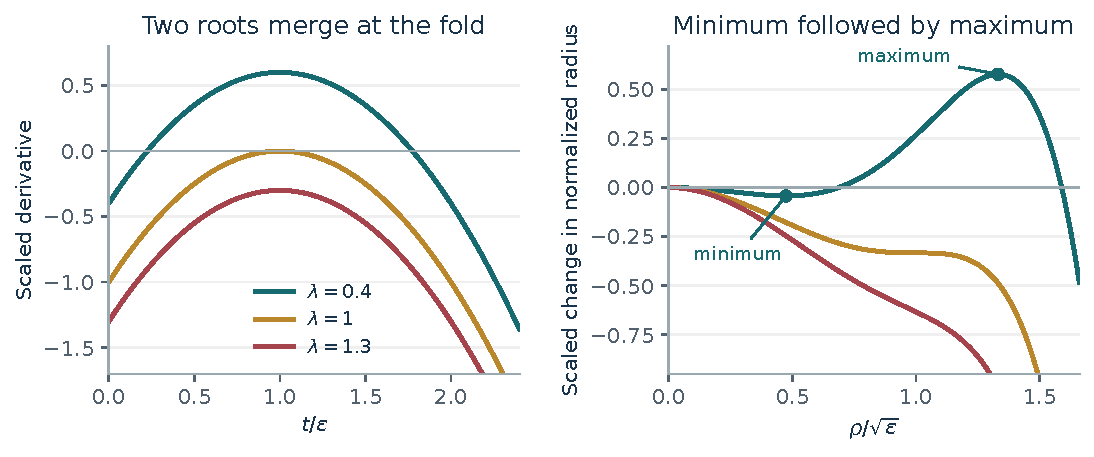
\includegraphics[width=\linewidth]{figures/radial_local_model.pdf}
\caption{The limiting local model on the paths
\eqref{turn:eq:scaling-path}. With $z=t/\varepsilon$ and
$u=\rho/\sqrt\varepsilon$, the scaled derivative is
$-\lambda+2z-z^2$ and the scaled change of normalized radius is
$-\lambda u^2+u^4-u^6/3$. The latter uses the positive scale
$-3R_0\varepsilon^3$. These are the proved leading local terms,
not direct numerical evaluations of the full function. The exact
fold has higher-order corrections to the displayed $\lambda=1$ model.}
\label{turn:fig:model}
\end{figure}

\subsection{What the result resolves and what remains}
\label{turn:sec:status}

The manuscript's displayed quartic-transition location is now replaced
by an exact rational enclosure, a local uniqueness theorem, a
transversality sign, and a negative sextic coefficient.  Its request
for the local higher-order radial behavior at that transition is
answered by Theorem~\ref{turn:thm:fold}.  The resulting region with a
minimum followed by a maximum is stronger than the preceding
existence results for one minimum or one maximum separately.

Three natural questions remain distinct.  First, is this the only
zero of $Q(a_*(b),b)$ in $0<b<1$?  Second, can one give explicit
numerical lower bounds for the parameter neighborhood and the fixed
radius $\sqrt T$ in the fold theorem?  Third, do the same parameter
pairs have additional turning points at larger radii?  The present
finite certificate answers none of these global or quantitative
questions by itself.  It establishes a nondegenerate local mechanism
that any proposed global classification must accommodate.

Another useful direction is the fully constant point $(a,b)=(1,1)$,
where $F_{1,1}(z)=\tfrac12\log^2(1-z)$ and
$\eta_{1,1}(\rho)=1/2$.  At that point every nonconstant radial
coefficient vanishes.  Relating that higher degeneracy to the nearby
certified fold requires further analysis; it cannot be inferred from
the sign of $R_0$ alone.  Proposition~\ref{turn:prop:recurrence}
provides an exact finite calculation at each order for such an
investigation.
